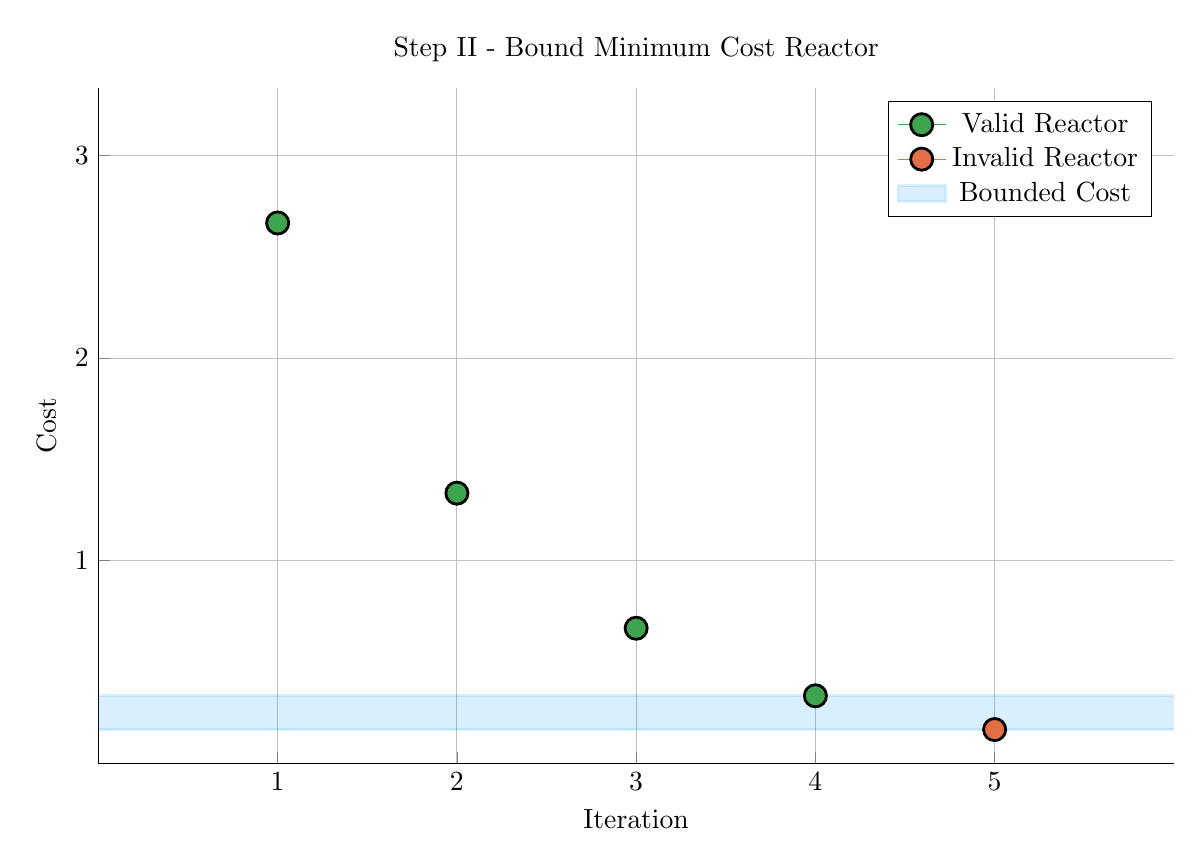
\begin{tikzpicture}[]
\begin{axis}[height = {101.6mm}, ylabel = {Cost}, title = {Step II - Bound Minimum Cost Reactor}, xmin = {0}, xmax = {6}, ymax = {40}, xlabel = {Iteration}, {unbounded coords=jump, xticklabel style={rotate = 0}, xmajorgrids = true, xtick = {1.0,2.0,3.0,4.0,5.0}, xticklabels = {1,2,3,4,5}, xtick align = inside, axis lines* = left, yticklabel style={rotate = 0}, ymajorgrids = true, ytick = {12,24,36}, yticklabels = {1,2,3}, ytick align = inside, axis lines* = left,     xshift = 0.0mm,
    yshift = 0.0mm,
    axis background/.style={fill={rgb,1:red,1.00000000;green,1.00000000;blue,1.00000000}}
}, ymin = {0}, width = {152.4mm}]\addplot+[draw=none, color = {rgb,1:red,0.24222430;green,0.64327509;blue,0.30444865},
draw opacity=1.0,
line width=0,
solid,mark = *,
mark size = 4.0,
mark options = {
    color = {rgb,1:red,0.00000000;green,0.00000000;blue,0.00000000}, draw opacity = 1.0,
    fill = {rgb,1:red,0.24222430;green,0.64327509;blue,0.30444865}, fill opacity = 1.0,
    line width = 1,
    rotate = 0,
    solid
}] coordinates {
(1.0, 32.0)
};
\addlegendentry{Valid Reactor}
\addplot+[draw=none, color = {rgb,1:red,0.24222430;green,0.64327509;blue,0.30444865},
draw opacity=1.0,
line width=0,
solid,mark = *,
mark size = 4.0,
mark options = {
    color = {rgb,1:red,0.00000000;green,0.00000000;blue,0.00000000}, draw opacity = 1.0,
    fill = {rgb,1:red,0.24222430;green,0.64327509;blue,0.30444865}, fill opacity = 1.0,
    line width = 1,
    rotate = 0,
    solid
},forget plot] coordinates {
(2.0, 16.0)
};
\addplot+[draw=none, color = {rgb,1:red,0.24222430;green,0.64327509;blue,0.30444865},
draw opacity=1.0,
line width=0,
solid,mark = *,
mark size = 4.0,
mark options = {
    color = {rgb,1:red,0.00000000;green,0.00000000;blue,0.00000000}, draw opacity = 1.0,
    fill = {rgb,1:red,0.24222430;green,0.64327509;blue,0.30444865}, fill opacity = 1.0,
    line width = 1,
    rotate = 0,
    solid
},forget plot] coordinates {
(3.0, 8.0)
};
\addplot+[draw=none, color = {rgb,1:red,0.24222430;green,0.64327509;blue,0.30444865},
draw opacity=1.0,
line width=0,
solid,mark = *,
mark size = 4.0,
mark options = {
    color = {rgb,1:red,0.00000000;green,0.00000000;blue,0.00000000}, draw opacity = 1.0,
    fill = {rgb,1:red,0.24222430;green,0.64327509;blue,0.30444865}, fill opacity = 1.0,
    line width = 1,
    rotate = 0,
    solid
},forget plot] coordinates {
(4.0, 4.0)
};
\addplot+[draw=none, color = {rgb,1:red,0.88887350;green,0.43564919;blue,0.27812294},
draw opacity=1.0,
line width=0,
solid,mark = *,
mark size = 4.0,
mark options = {
    color = {rgb,1:red,0.00000000;green,0.00000000;blue,0.00000000}, draw opacity = 1.0,
    fill = {rgb,1:red,0.88887350;green,0.43564919;blue,0.27812294}, fill opacity = 1.0,
    line width = 1,
    rotate = 0,
    solid
}] coordinates {
(5.0, 2.0)
};
\addlegendentry{Invalid Reactor}
\addplot+ [color = {rgb,1:red,0.00000000;green,0.60560316;blue,0.97868012},
draw opacity=0.15,
line width=1,
solid,mark = none,
mark size = 2.0,
mark options = {
    color = {rgb,1:red,0.00000000;green,0.00000000;blue,0.00000000}, draw opacity = 0.15,
    fill = {rgb,1:red,0.00000000;green,0.60560316;blue,0.97868012}, fill opacity = 0.15,
    line width = 1,
    rotate = 0,
    solid
},fill = {rgb,1:red,0.00000000;green,0.60560316;blue,0.97868012}, fill opacity=0.15,area legend]coordinates {
(-1.0, 4.0)
(-1.0, 2.0)
(7.0, 2.0)
(7.0, 4.0)
(-1.0, 4.0)
};
\addlegendentry{Bounded Cost}
\end{axis}

\end{tikzpicture}
